% 问题三
\section{问题三：通信约束下运输与中继联合调度}
\label{sec:p3}

\subsection{问题分析}

第五节给出了纯运输调度方案，但未考虑通信约束。题目要求无人机整个飞行过程与
调度中心保持通信，可行方式为直连或经悬停中继的双跳。镇龙乡山高谷深，低空
作业段与穿越山谷的巡航段极易被山体遮挡，直连无法全程成立，需在合适位置布设
中继并安排其工作时段。因此问题三需要将运输调度与中继布设调度联合优化：
中继位置决定哪些时段必须中继，运输架次的时刻安排必须与中继服务窗口相容，
反之中继架次也要在能源预算内覆盖全部必要时段。

\subsection{通信链路模型}

\subsubsection{自由空间损耗与链路预算}

工作频率 $f=2400$\,MHz，收发间三维距离
$D=\sqrt{d_{\mathrm{2D}}^2+\Delta z^2}$，单位公里，自由空间损耗按式
\eqref{eq:fspl} 计算\cite{refITU}。

\begin{equation}
L_{\mathrm{FSPL}}=32.45+20\lg f_{\mathrm{MHz}}+20\lg D_{\mathrm{km}}
\label{eq:fspl}
\end{equation}

接收功率为发射功率减去自由空间损耗、系统损耗与遮挡损耗三项。通信有效需接收
功率不低于接收门限 $P_{\mathrm{th}}=P_{\mathrm{sens}}+M=-98+8=-90$\,dBm，
等价于链路总损耗不超过上限，即直连 122\,dB、经中继的接入链路 116\,dB、
中继到 O01 的回程链路 126\,dB。由式 \eqref{eq:fspl} 反解，三档上限对应的
最大三维距离约为 12.5、6.3、10.7\,km。

\subsubsection{地形遮挡判定}

对任意收发对，沿连线按 30\,m 步长采样，读取数字高程并与连线高度比较：任一
采样点地形高于连线则视距被遮挡，追加 10\,dB 遮挡损耗并判链路无效。无人机
位置沿其四维轨迹生成，即时间、经度、纬度、高度，故覆盖判定是确定性的。

\subsection{中继布设}

以覆盖采样法确定候选布设位置：对全部架次轨迹采样点先判直连有效，直接排除；
对直连失败点在若干地形高点候选位逐一检验接入链路与回程链路是否同时成立。
结果表明三个布设点即可覆盖全部需中继时段，其坐标如下。

\begin{itemize}
\item 西点 $P_W=(109.2103^{\circ}\mathrm{E},\,23.0471^{\circ}\mathrm{N},\,
676.5\,\mathrm{m})$：覆盖西与北片区，即 S001、S002、S003、S005、S007、
S008、S009、S011、S015 及其转运走廊；
\item 东点 $P_E=(109.2689^{\circ}\mathrm{E},\,23.0127^{\circ}\mathrm{N},\,
650.0\,\mathrm{m})$：覆盖东片区，即 S010、S012、S013、S014；
\item 北点 $P_N=(109.2343^{\circ}\mathrm{E},\,23.0592^{\circ}\mathrm{N},\,
600.0\,\mathrm{m})$：覆盖 S004 及经过其走廊的深入航线，因 S004 直连不可达
必须经中继。
\end{itemize}

三个布设点与服务区的地理聚类一致，即西与北九区、东四区、S004 独点，
为第\ref{sec:p4}节的分区提供了依据。图 \ref{fig:p3cov} 给出布设点与
6.3\,km 接入半径示意。

\begin{figure}[htbp]
\centering
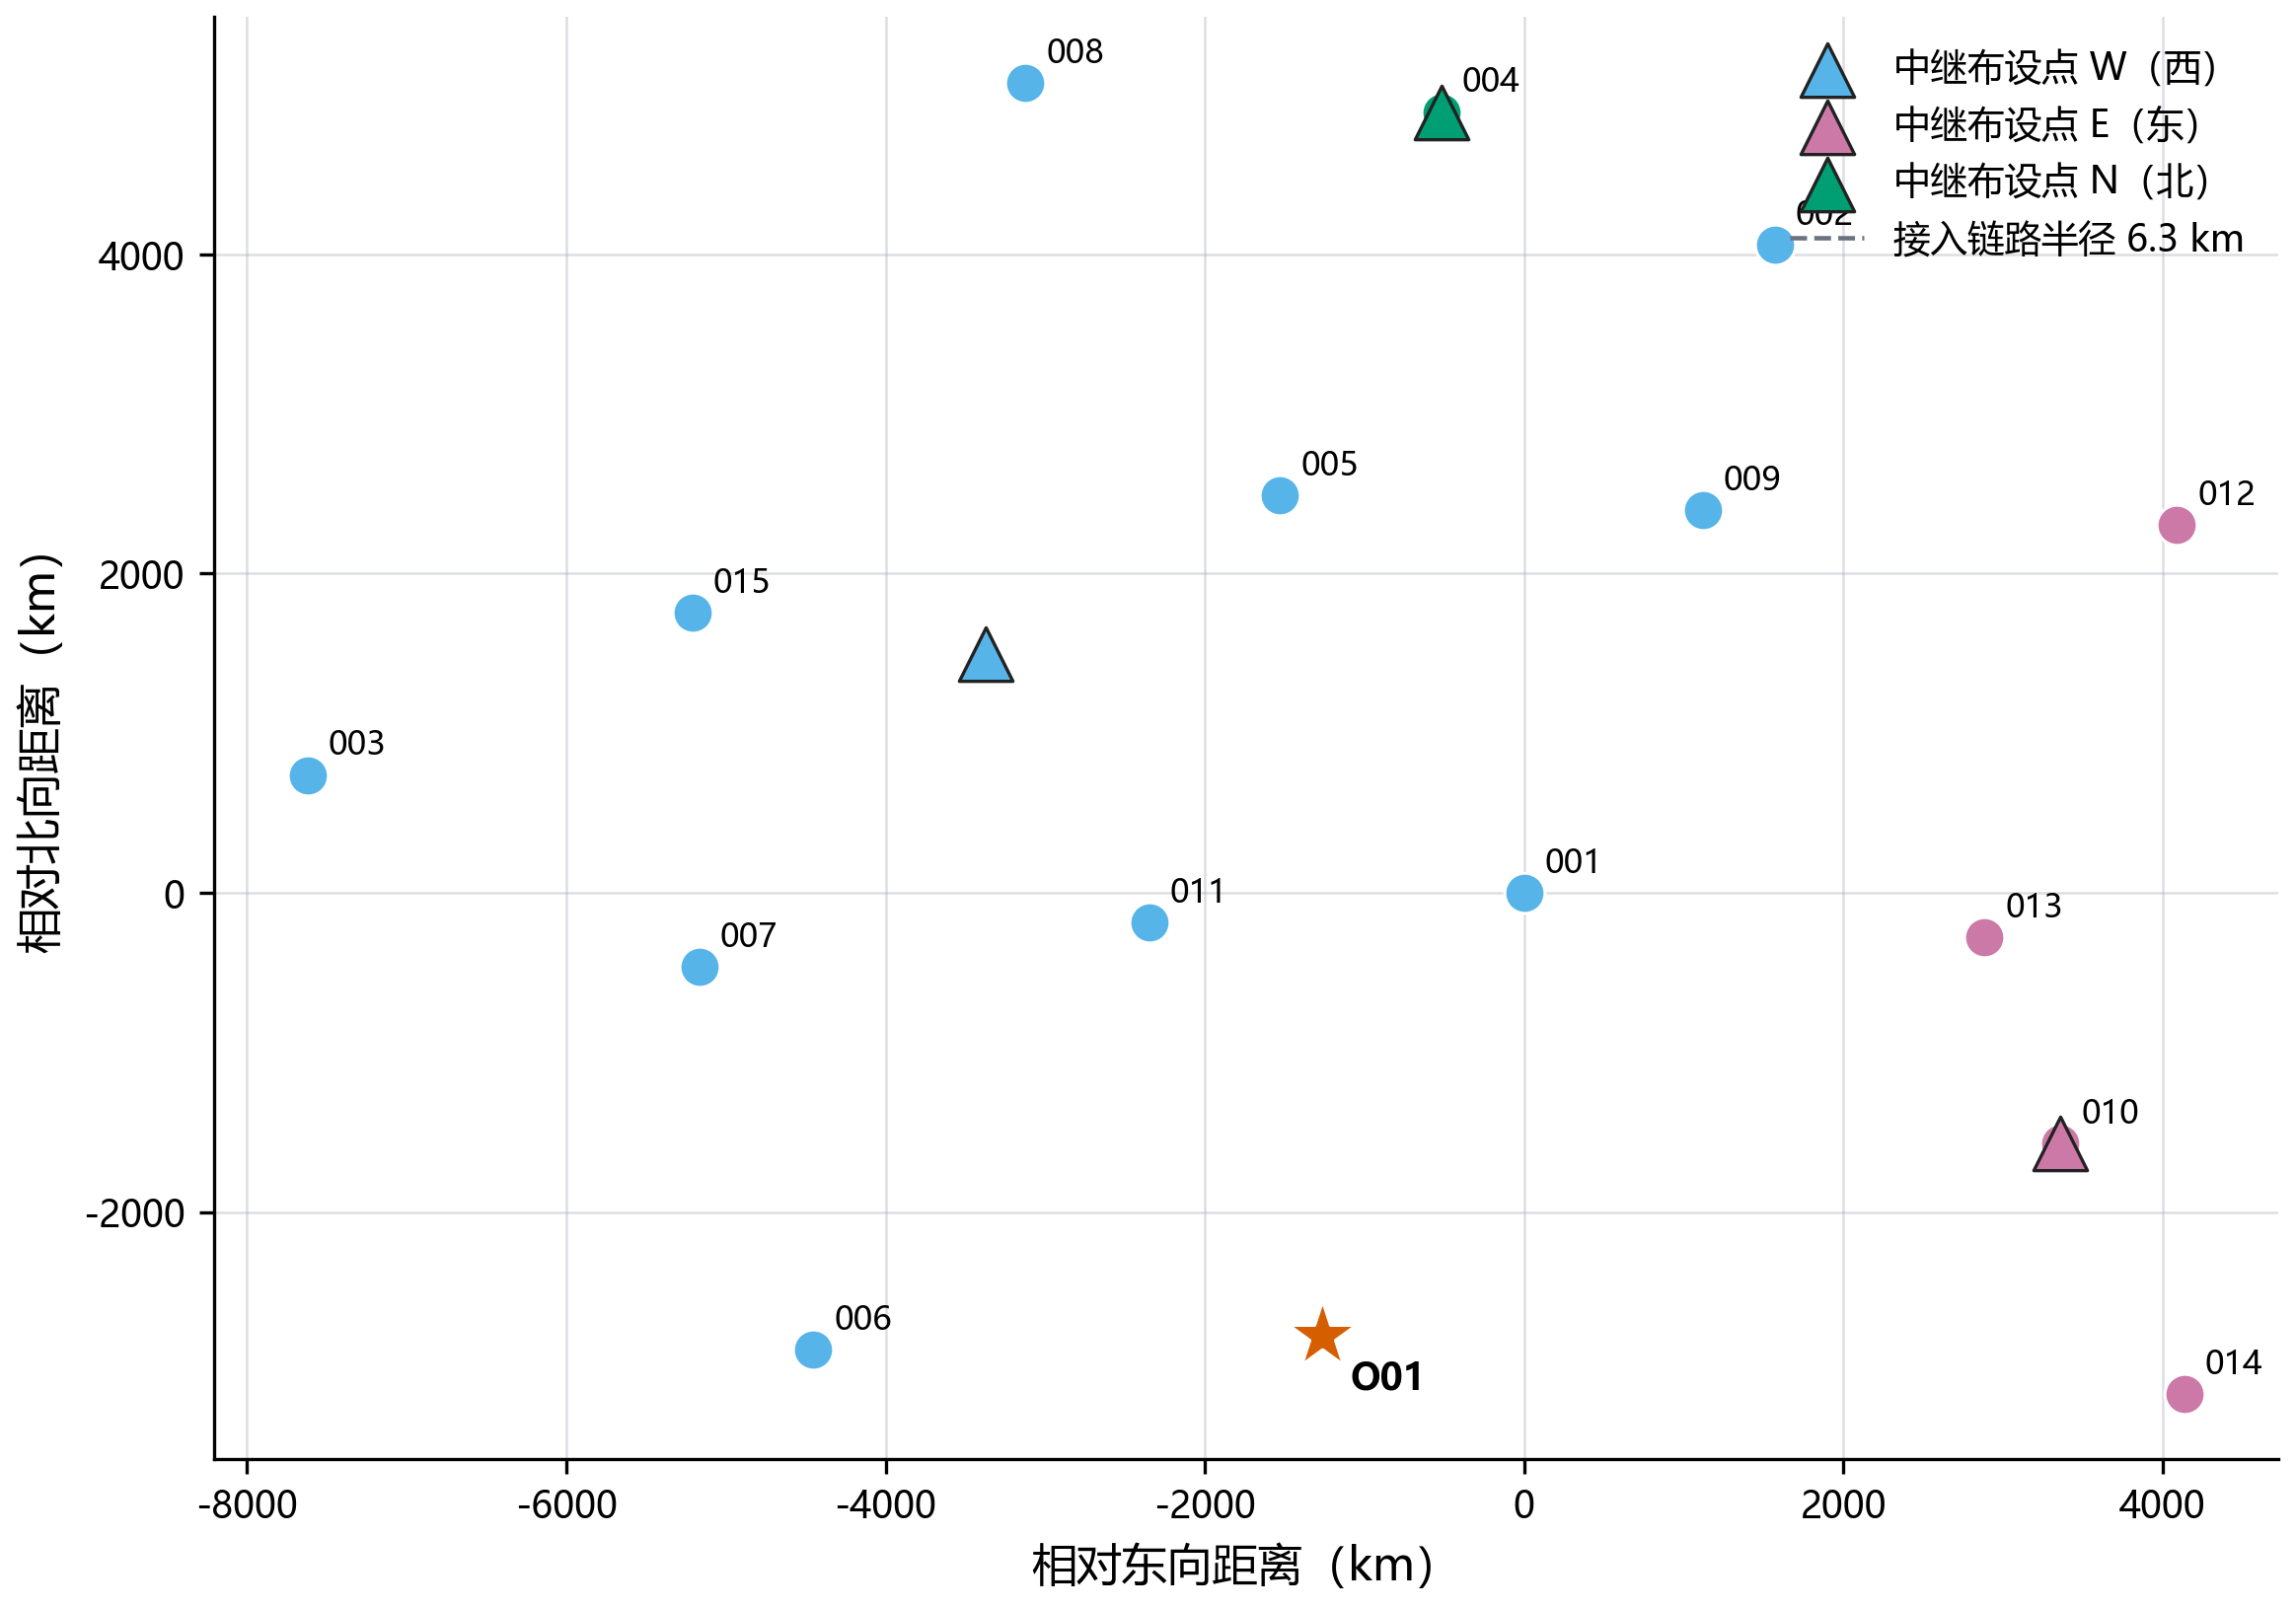
\includegraphics[width=0.76\textwidth]{figures/p3_coverage.png}
\caption{三个中继布设点及其接入链路半径示意（虚线圆半径 6.3 km）}
\label{fig:p3cov}
\end{figure}

\subsection{运输与中继的联合调度}

\subsubsection{逐区段通信判定}

对每个架次，沿轨迹对服务区作业段与相邻转运段逐点判定：直连有效者保持直连；
直连失败者分配给某一中继布设点，要求接入与回程链路同时满足，且该点当前处于
服务窗口。任一采样点无可用链路即记为盲区。覆盖判定对全部架次轨迹执行，得到
每个需中继的飞行阶段、其归属布设点与起止时刻，作为中继排班的输入。

\subsubsection{覆盖审核与中继时序规划}

对第五节选区的 28 架次区一致方案按 30\,m 步长做通信审核，得到 1762 个需中继采样点。
初始中继布设即实现全覆盖：西点、东点与北点三个布设点的接入与回程链路在全部采样点
均可行，初始方案未做人工调整。中继单架次能源预算为 $(1-\rho)E_{\mathrm{use}}=2.56$\,kWh，
三班均未超预算。

最终两架中继的时间分片方案如下：
\begin{itemize}
\item 中继 1 驻西点，服务时段 [1058, 7453]\,s，能耗 2.184\,kWh，返航荷电状态约
$1-2.184/3.2=31.8\%$，高于 20\% 的安全下限；
\item 中继 2 先驻东点，服务时段 [1060, 5498]\,s，能耗 1.549\,kWh；再返航换装满充组件并转场北点，
服务时段 [6565, 7308]\,s，能耗 0.488\,kWh；最后转场西点承担 W 尾段 [8605, 9072]\,s，
能耗 0.372\,kWh。三个时段窗口不重叠，转场衔接经严格口径核算仅有 58\,s 转场等待。
\end{itemize}

按题目附录 2 的严格口径复核：每次任务含 180\,s 起飞准备、30\,s
建链与 300\,s 架次周转；能源组件复用前必须充满（初始 SOC 为 100\%，用后按
两阶段曲线充至 100\%）。东点班返航荷电约 $1-1.549/3.2=51.6\%$，北点班取自
6 组件共享池内的满充新组件，不受东点班组件充电进度约束；北点班派单 6100\,s
与东点班返场 5857\,s 间隔 243\,s，西点尾段班派单 8182\,s 与北点班返场 7763\,s
间隔 419\,s，经组件池就绪时间核算仅产生 58\,s 的转场
等待（machine\_pen$=58$\,s），不影响各窗口中继覆盖。西点需求总时长约 8014\,s，
单班服务能耗将超过 2.56\,kWh 的能源预算，故拆为 W1 与 W2 两班，间隙 1152\,s
用于中继转场与组件轮换。中继最晚返场为西点尾段班 9491\,s，晚于运输侧偏移后
完工约 9473\,s，故联合任务完工时间由中继 1 尾段班返场决定，
为 9491\,s（约 158.2\,min）。

需中继采样点按布设点归属的空间分布见图 \ref{fig:relaycover}：西片区与北部
走廊归西点、东片区归东点、S004 走廊归北点，三组聚类清晰、无重叠，构成问题四
任务分区的地理基础。

\begin{figure}[htbp]
\centering
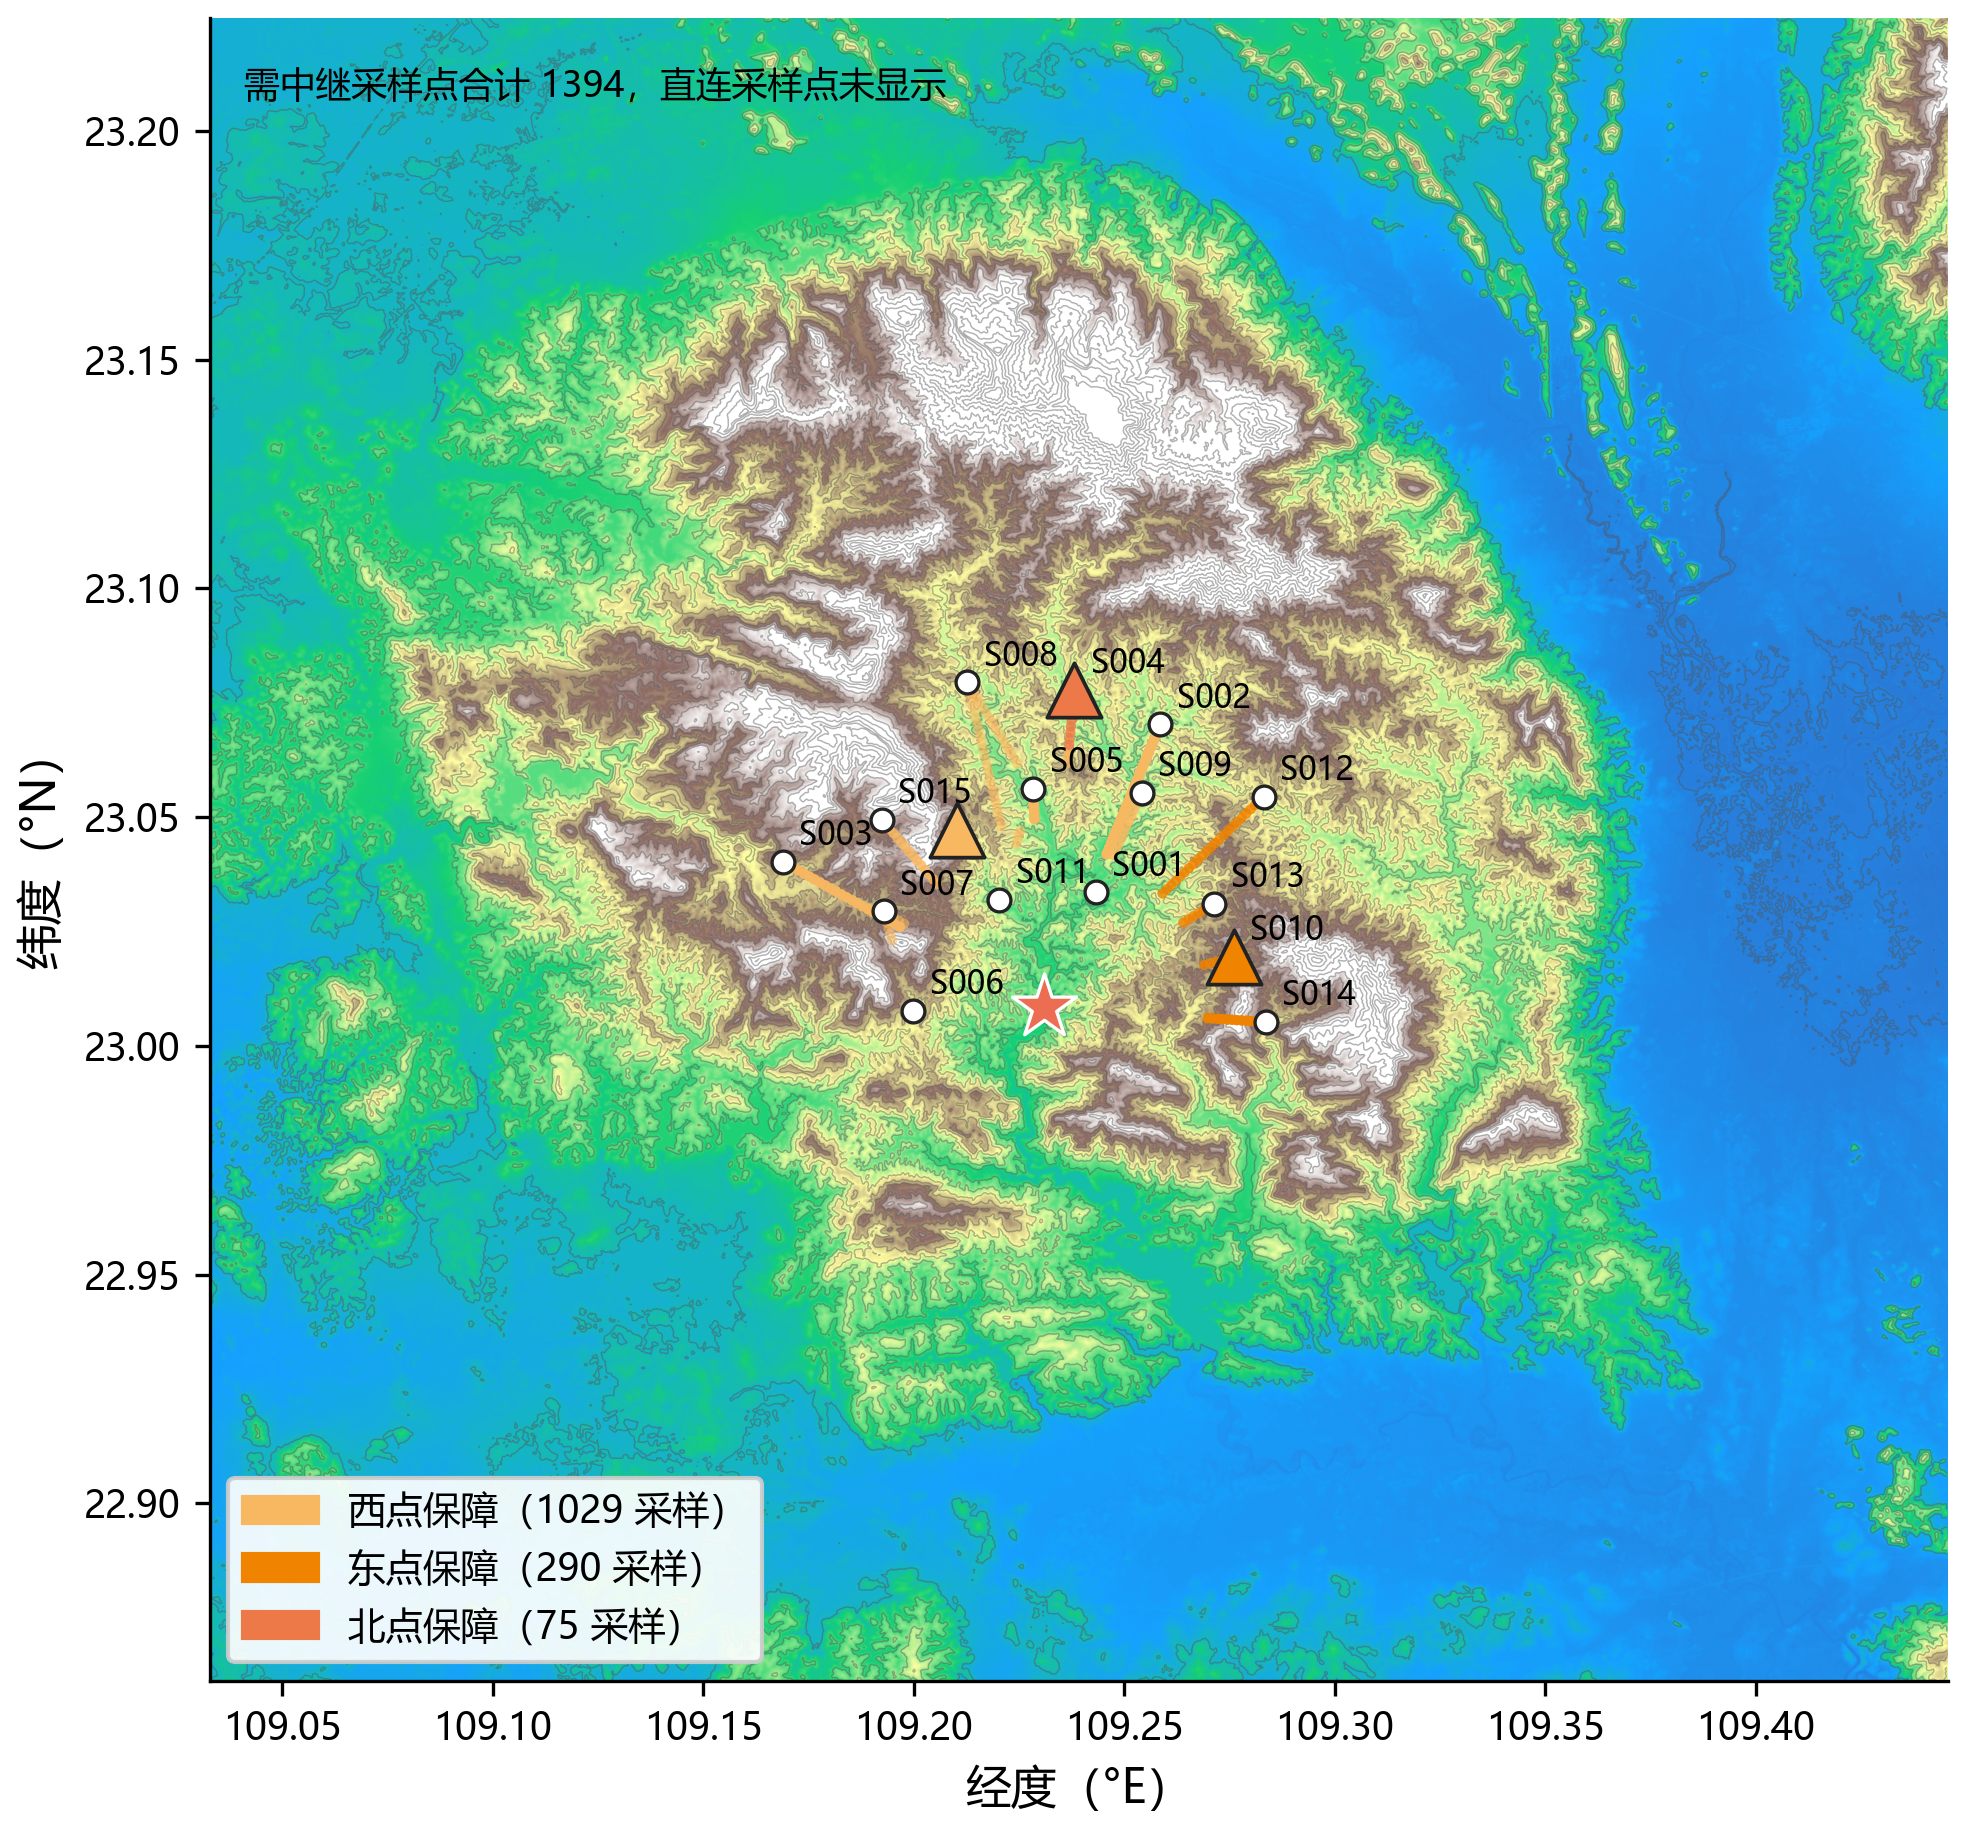
\includegraphics[width=0.96\textwidth]{figures/p3_relay_coverage.png}
\caption{1762 个需中继采样点按布设点的归属分布（DEM 底图）}
\label{fig:relaycover}
\end{figure}

中继架次明细见表 \ref{tab:relay}，图 \ref{fig:relaytl} 给出两架中继四个服务时段的时间线。

\begin{figure}[htbp]
\centering
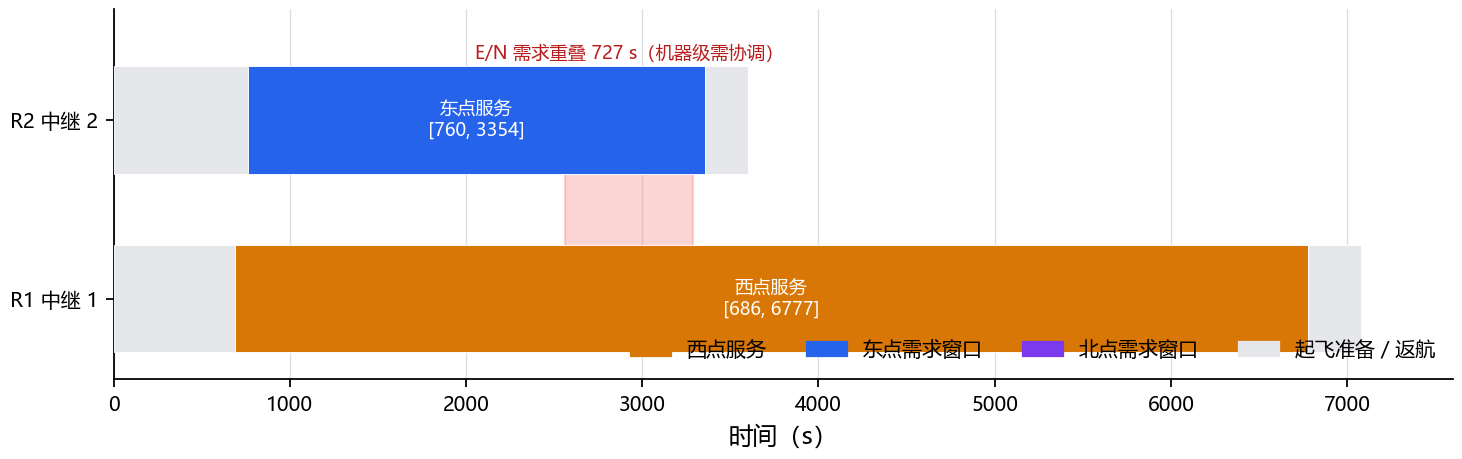
\includegraphics[width=0.98\textwidth]{figures/p3_relay_tl.png}
\caption{两架中继四个服务时段的时间线（浅灰为起飞准备与返航）}
\label{fig:relaytl}
\end{figure}

\begin{table}[htbp]
\centering
\caption{中继架次安排（中继 1 驻西点，中继 2 依次东点、北点、西点尾段）}
\label{tab:relay}
\begin{tabular}{ccccccc}
\toprule
中继架次 & 无人机 & 能源组件 & 任务位置 & 服务时段(s) & 能耗(kWh) & 覆盖状态 \\
\midrule
R1-01 & 中继1 & 组件1 & 西点 & [1058, 7453] & 2.184 & 全覆盖 \\
R1-02 & 中继1 & 组件2 & 西点 & [8605, 9072] & 0.372 & 全覆盖 \\
R2-01 & 中继2 & 组件3 & 东点 & [1060, 5498] & 1.549 & 全覆盖 \\
R2-02 & 中继2 & 组件4 & 北点 & [6565, 7308] & 0.488 & 全覆盖 \\
\bottomrule
\end{tabular}
\end{table}

\subsection{联合调度结果}

协同后的运输方案仍为 28 架次区一致方案（与第五节一致），全部货箱按时投送至
各自指定服务区（三档时限零违反、加权迟到为零）。通信方面，
西点两班与东、北两班中继分别承担 2.184、0.372、1.549 与 0.488\,kWh，
中继合计约 4.59\,kWh；
自动化覆盖诊断确认初始布设即全覆盖（1762 个需中继采样点零未覆盖），
中继四班均满足能源预算，东转北衔接经组件池严格口径核算仅 58\,s 转场等待。为
对齐中继时窗，对需北点覆盖的 S004 所属架次施加后移偏移（f22 约 2100\,s），
带动相关链小幅顺延，偏移后运输完工约 9473\,s；中继 1 西点尾段班最晚返场
9491\,s 决定联合完工——中继约束引入的
完工代价约 2096\,s（较纯运输 7395\,s，约 28.3\%），集中于北点窗口与西点长班
覆盖的必要等待。
表 \ref{tab:p3cmp} 给出与纯运输方案的指标对比，图 \ref{fig:p3gantt}
给出运输与中继的联合甘特图。图 \ref{fig:commtl} 给出每个运输架次的通信
保障方式时间线，浅灰段为直连，彩色段为中继，可见需中继的时段集中于西与北
片区作业段与 S004 走廊，且全部落在对应中继的服务窗口内；架次明细见表
\ref{tab:p3flights}。

\begin{figure}[htbp]
\centering
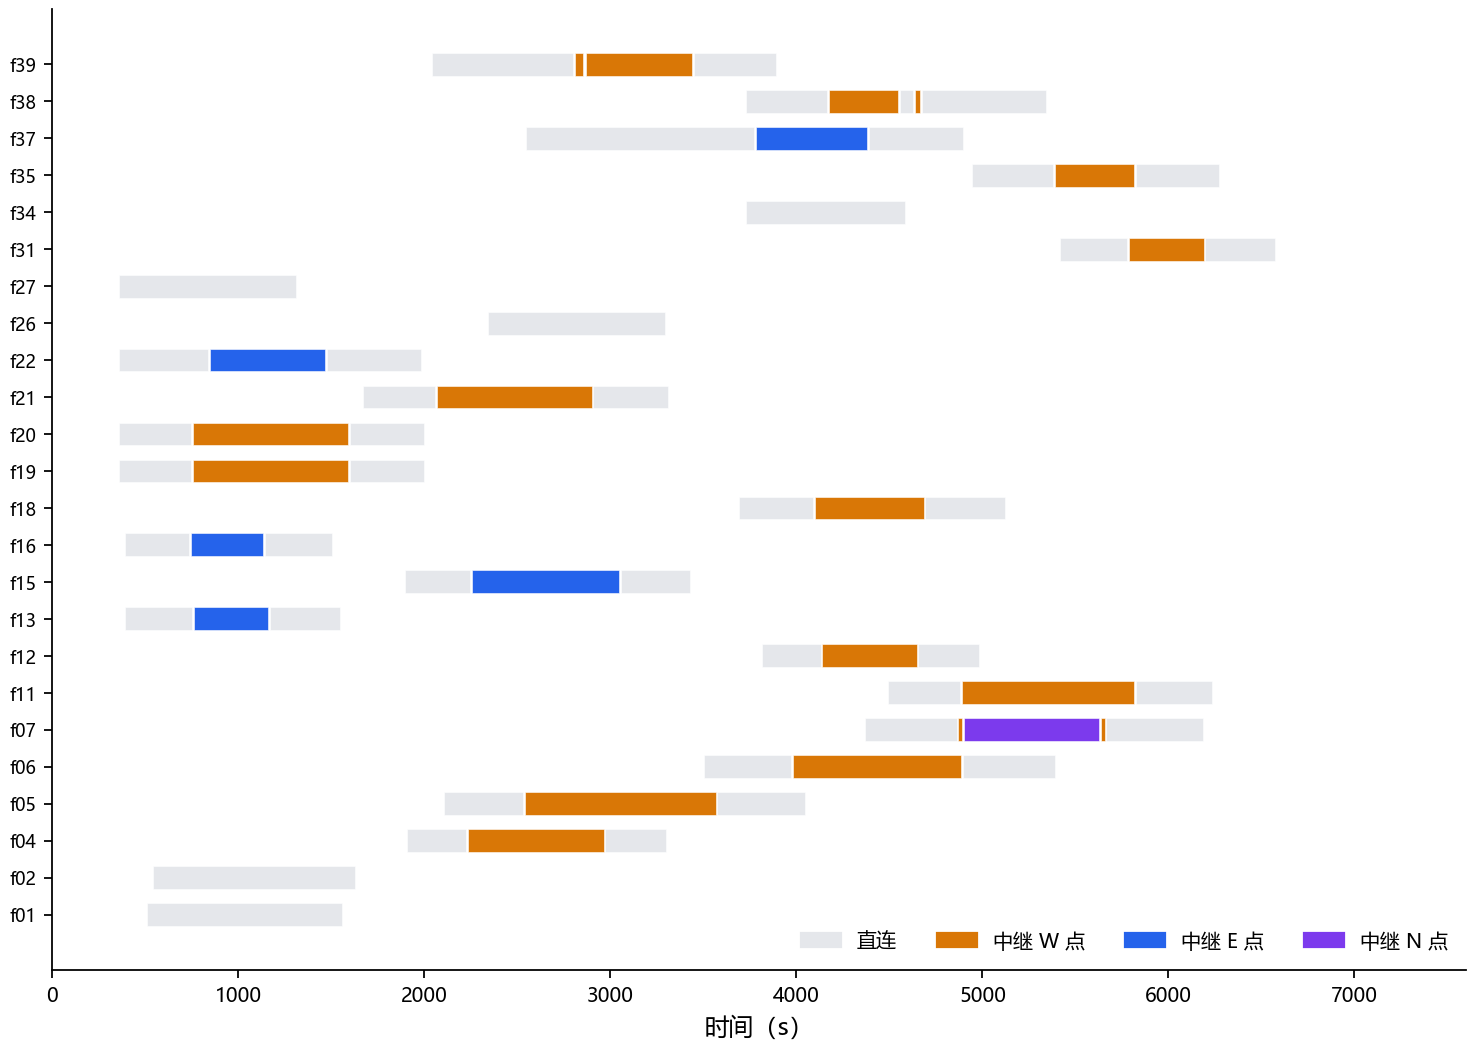
\includegraphics[width=0.98\textwidth]{figures/p3_comm_tl.png}
\caption{各运输架次的通信保障方式时间线（浅灰为直连，彩色为中继）}
\label{fig:commtl}
\end{figure}

\begin{table}[htbp]
\centering
\caption{问题三协同方案主要指标（与问题二对比）}
\label{tab:p3cmp}
\begin{tabular}{lccc}
\toprule
指标 & 问题二（纯运输） & 问题三（协同） & 变化 \\
\midrule
架次数 & 28 & 28 & 不变 \\
完工时间(s) & 7395 & 9491 & 中继尾段班返场 +2096（28.3\%） \\
运输能耗(kWh) & 83.12 & 83.12 & 不变 \\
中继能耗(kWh) & 未计 & 4.59 & 四班保障 \\
通信盲区 & 未计 & 0 & 初始布设即全覆盖 \\
中继架次 & 无 & 4 时段 & 两架分片复用 \\
\bottomrule
\end{tabular}
\end{table}

\begin{figure}[htbp]
\centering
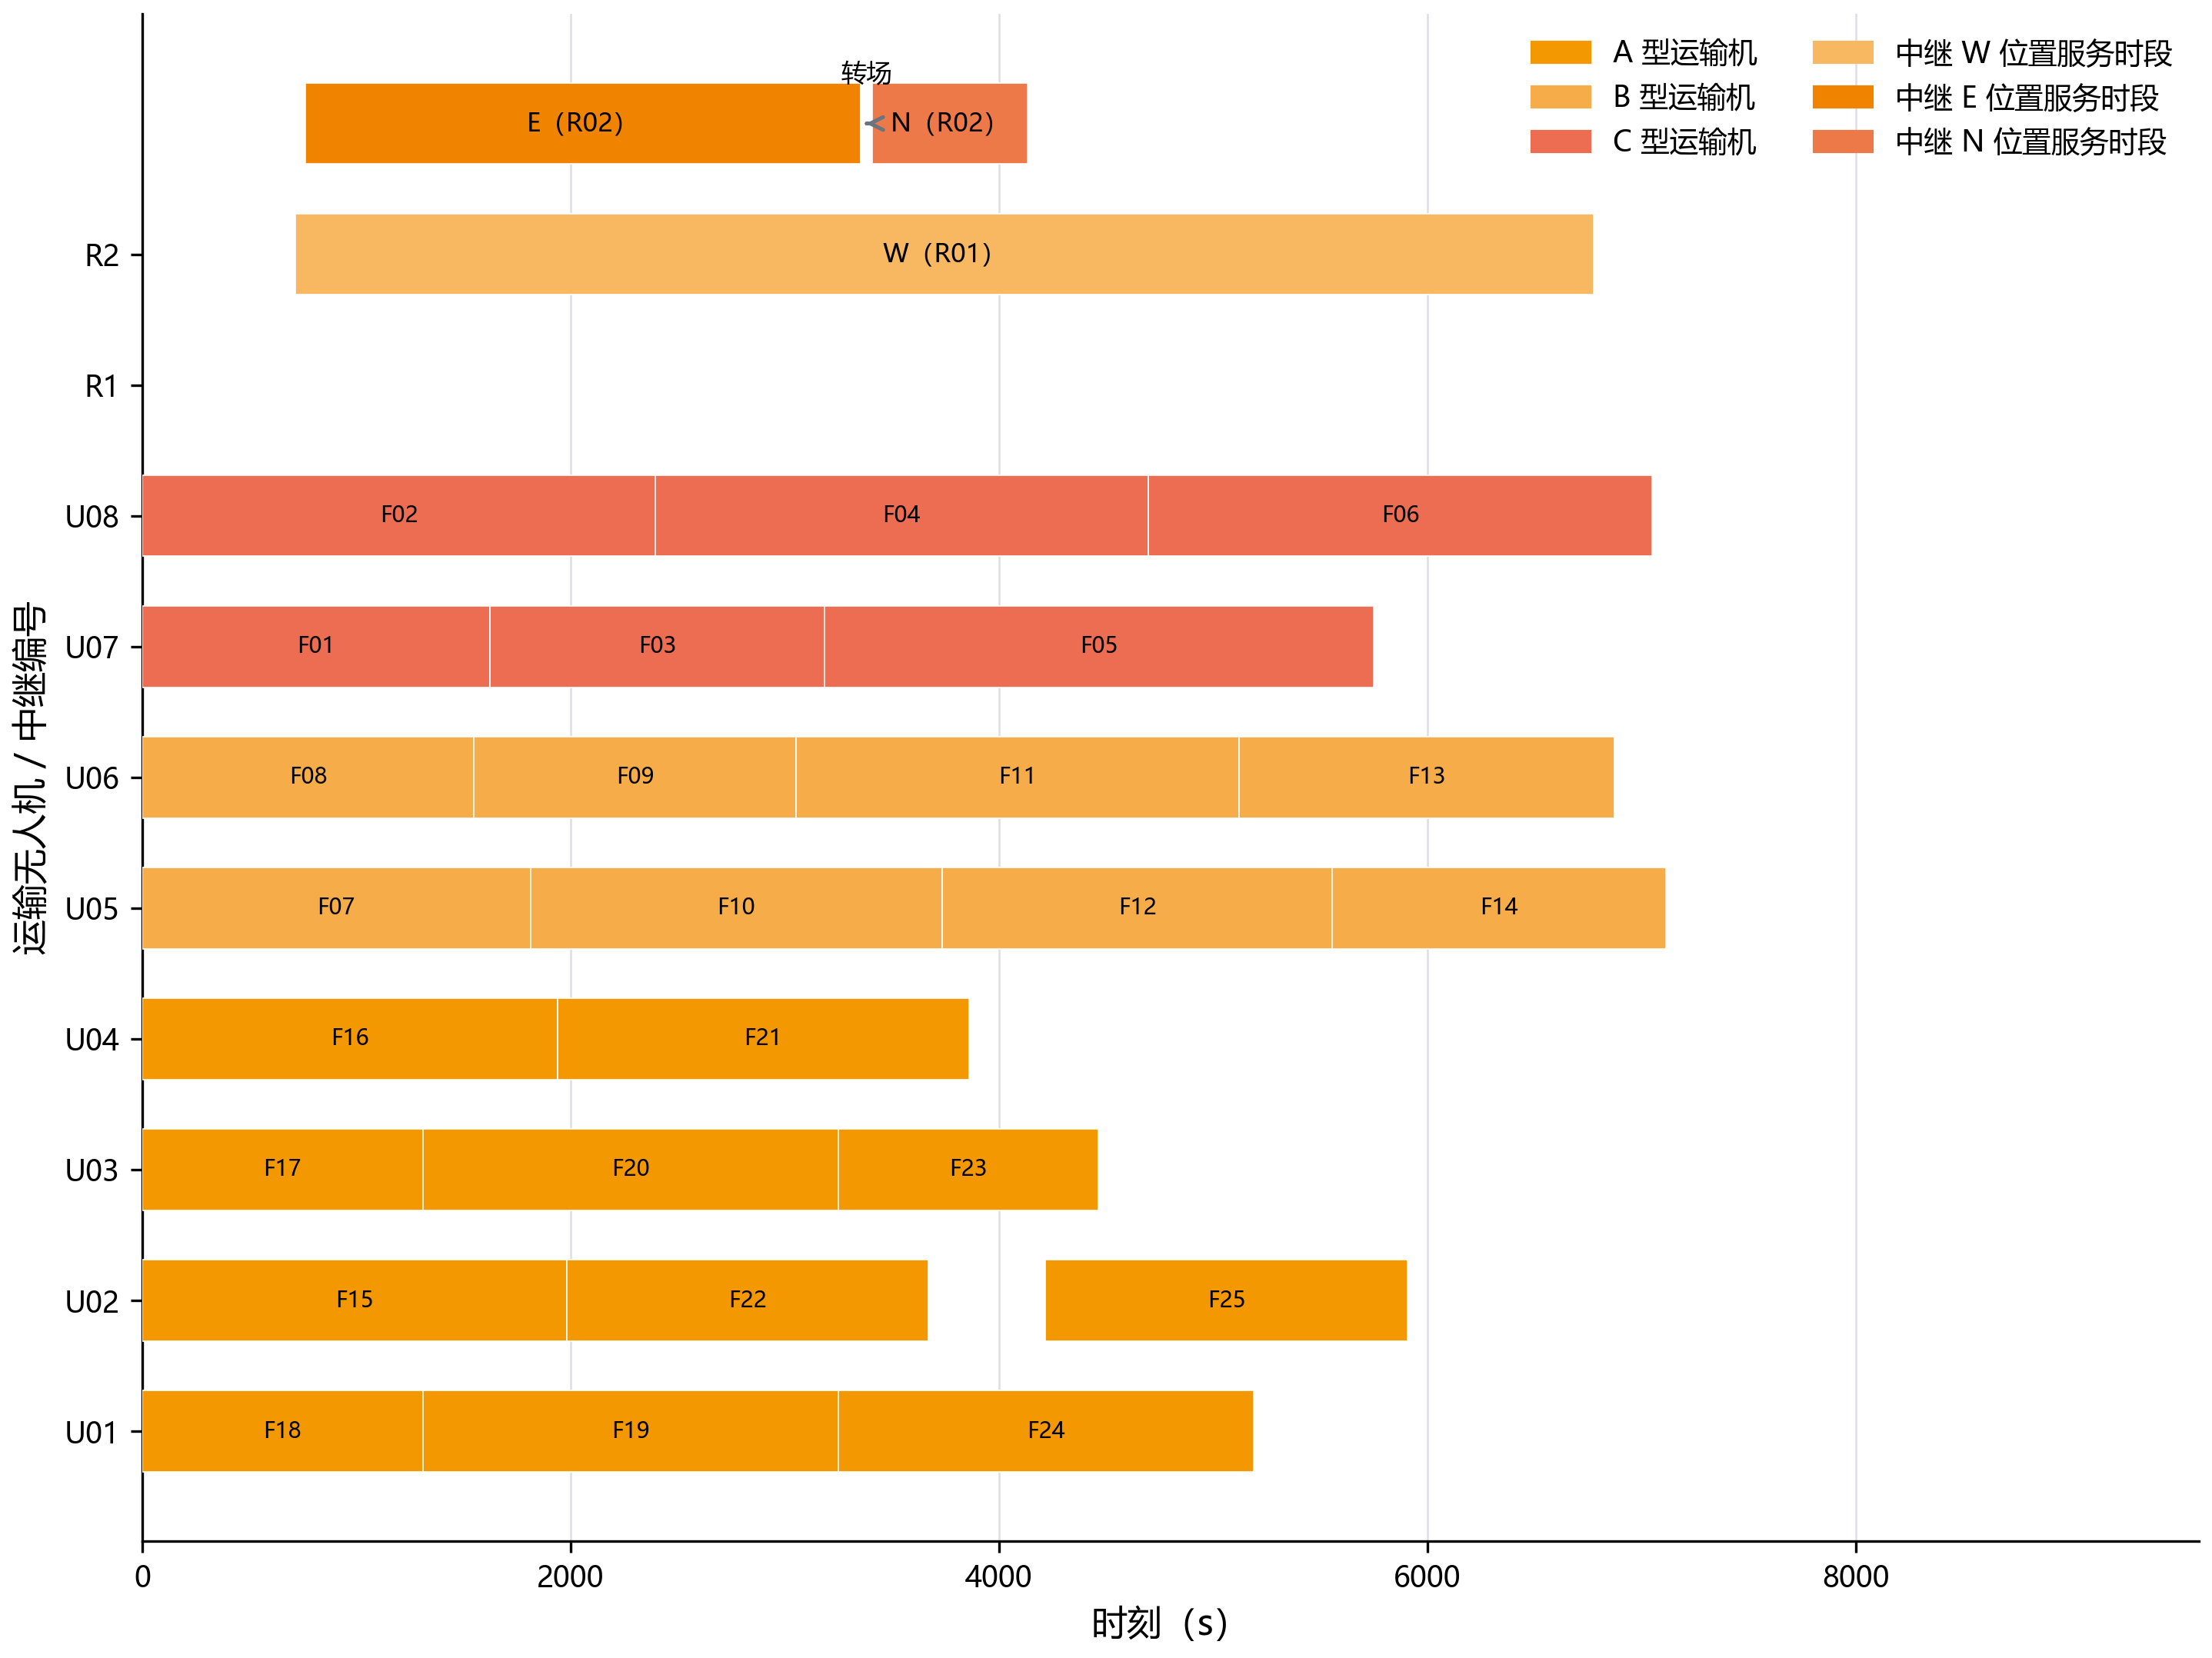
\includegraphics[width=0.98\textwidth]{figures/p3_gantt.png}
\caption{运输与中继协同调度甘特图（上：8 架运输机；下：中继 1 与中继 2 时段）}
\label{fig:p3gantt}
\end{figure}

\begin{table}[htbp]
\centering
\caption{问题三协同方案架次明细（28 架次，时刻为对齐中继窗口后的偏移派单）}
\label{tab:p3flights}
\small
\begin{tabular}{ccccccc}
\toprule
架次 & 机型 & 无人机 & 开始(s) & 返回(s) & 能耗(kWh) & 航线 \\
\midrule
f16 & C & U07 & 300 & 1858 & 2.99 & S001 \\
f24 & C & U08 & 300 & 1791 & 2.36 & S006 \\
f17 & C & U08 & 1791 & 3218 & 2.40 & S001 \\
f18 & C & U07 & 1858 & 3895 & 5.71 & S002 \\
f03 & C & U08 & 3218 & 5639 & 5.89 & S003 \\
f26 & C & U08 & 5639 & 7694 & 5.39 & S008 \\
f22 & C & U07 & 5700 & 7867 & 5.51 & S004 \\
f23 & C & U08 & 7863 & 9473 & 3.46 & S005 \\
\midrule
f10 & B & U05 & 300 & 2407 & 2.27 & S010至S014 \\
f25 & B & U06 & 300 & 1921 & 1.77 & S007 \\
f12 & B & U06 & 1921 & 3842 & 2.75 & S012 \\
f07 & B & U05 & 2407 & 4433 & 2.15 & S007至S015 \\
f09 & B & U06 & 3842 & 5866 & 2.79 & S002至S009 \\
f11 & B & U05 & 4433 & 6346 & 2.46 & S013至S011 \\
f05 & B & U06 & 5866 & 7302 & 1.74 & S009 \\
f29 & B & U05 & 6346 & 7408 & 0.89 & S011 \\
\midrule
f01 & A & U01 & 300 & 1609 & 1.26 & S001 \\
f14 & A & U03 & 300 & 2281 & 2.29 & S014 \\
f36 & A & U02 & 300 & 1906 & 1.95 & S013 \\
f39 & A & U04 & 300 & 2728 & 3.28 & S002至S005 \\
f02 & A & U01 & 1609 & 4038 & 3.22 & S002至S005 \\
f06 & A & U02 & 1906 & 4270 & 2.85 & S006至S015 \\
f08 & A & U04 & 2728 & 4889 & 3.19 & S008 \\
f21 & A & U01 & 4038 & 6288 & 3.08 & S003 \\
f28 & A & U02 & 4270 & 6755 & 3.40 & S010至S005 \\
f15 & A & U04 & 5109 & 7606 & 3.17 & S015至S005 \\
f04 & A & U03 & 5581 & 7758 & 3.08 & S004 \\
f37 & A & U01 & 6288 & 7940 & 1.80 & S007 \\
\bottomrule
\end{tabular}
\end{table}

\subsection{结果分析}

\begin{enumerate}
\item \textbf{通信保障以可核验的完工代价换取全程无盲区}：为对齐中继时窗，
S004 所属架次后移约 2100\,s 并带动相关链顺延，运输完工由纯运输的 7395\,s 变为
偏移后约 9473\,s；中继 1 西点尾段班返场 9491\,s 成为联合完工口径，较运输再增约
18\,s。中继约束引入的完工代价约 2096\,s（28.3\%），集中于北点窗口必须覆盖的
S004 走廊与西点长班保障；运输能耗 83.12\,kWh 与问题二持平，中继四班新增能耗
约 4.59\,kWh。代价可进一步由运输层面向中继窗口的联合排程压缩（见第
\ref{sec:sens}节讨论），但零盲区与零迟到在严格口径下始终成立。
\item \textbf{两架中继即可全程保障}：中继 1 驻西点，中继 2 先东、后北、再西点尾段的
分片复用，使四个服务时段由两架中继在时间上错峰满足。28 架次将任务分散为
更多短架次，中继窗口随之缩短：西点两班 2.184 与 0.372\,kWh、东点 1.549\,kWh、
北点 0.488\,kWh，合计较任务集中为少数长班次的对照排班方式显著下降。
\item \textbf{能源预算自洽}：西点需求总时长约 8014\,s，单班服务能耗将超过
2.56\,kWh 预算，故拆为 W1（106.6\,min 连续服务、能耗 2.184\,kWh、返航荷电
31.8\%）与 W2（能耗 0.372\,kWh）两班，班间间隙 1152\,s 供中继返场与组件轮换，
6 组能源组件足以支持；东点、北点单班能耗分别 1.549 与 0.488\,kWh，返航荷电
51.6\% 与 84.8\%，余量充足。
\item \textbf{S004 的独特地位}：S004 直连与东西两点均无法覆盖，必须由北点
中继（[6565, 7308]\,s 服务窗口，全部对应 S004 走廊），其余运输任务都不会
进入北点窗口，因此北点时段为 S004 专属；这同时决定了第\ref{sec:p4}节中
S004 独立成组的必要性。
\end{enumerate}